\begin{frame}
    \begin{center}
        \Huge Categorical Neural Networks
    \end{center}
\end{frame}

\begin{frame}{The idea of categorical neural networks}
    \begin{itemize}
        \item \Large Difficult backgrounds $\rightarrow$ additional targets
    \end{itemize}
\end{frame}

\begin{frame}{Target handling}
    \begin{itemize}
        \item Using One-Hot-Encoding
        \vspace{0.23cm}
        \item Vector instead of target
        \vspace{0.23cm}
        \item Target values get translated to vector component
    \end{itemize}
    \vspace{0.23cm}
    \begin{equation*}
    \tHq = \begin{bmatrix}
           0 \\
           0 \\
           1
         \end{bmatrix}
    \tZq = \begin{bmatrix}
           1 \\
           0 \\
           0
         \end{bmatrix}
    Background = \begin{bmatrix}
           0 \\
           1 \\
           0
         \end{bmatrix}
    \end{equation*}
\end{frame}

\begin{frame}{Binary final node - Sigmoid}
    \begin{columns}
        \begin{column}{0.65\textwidth}
            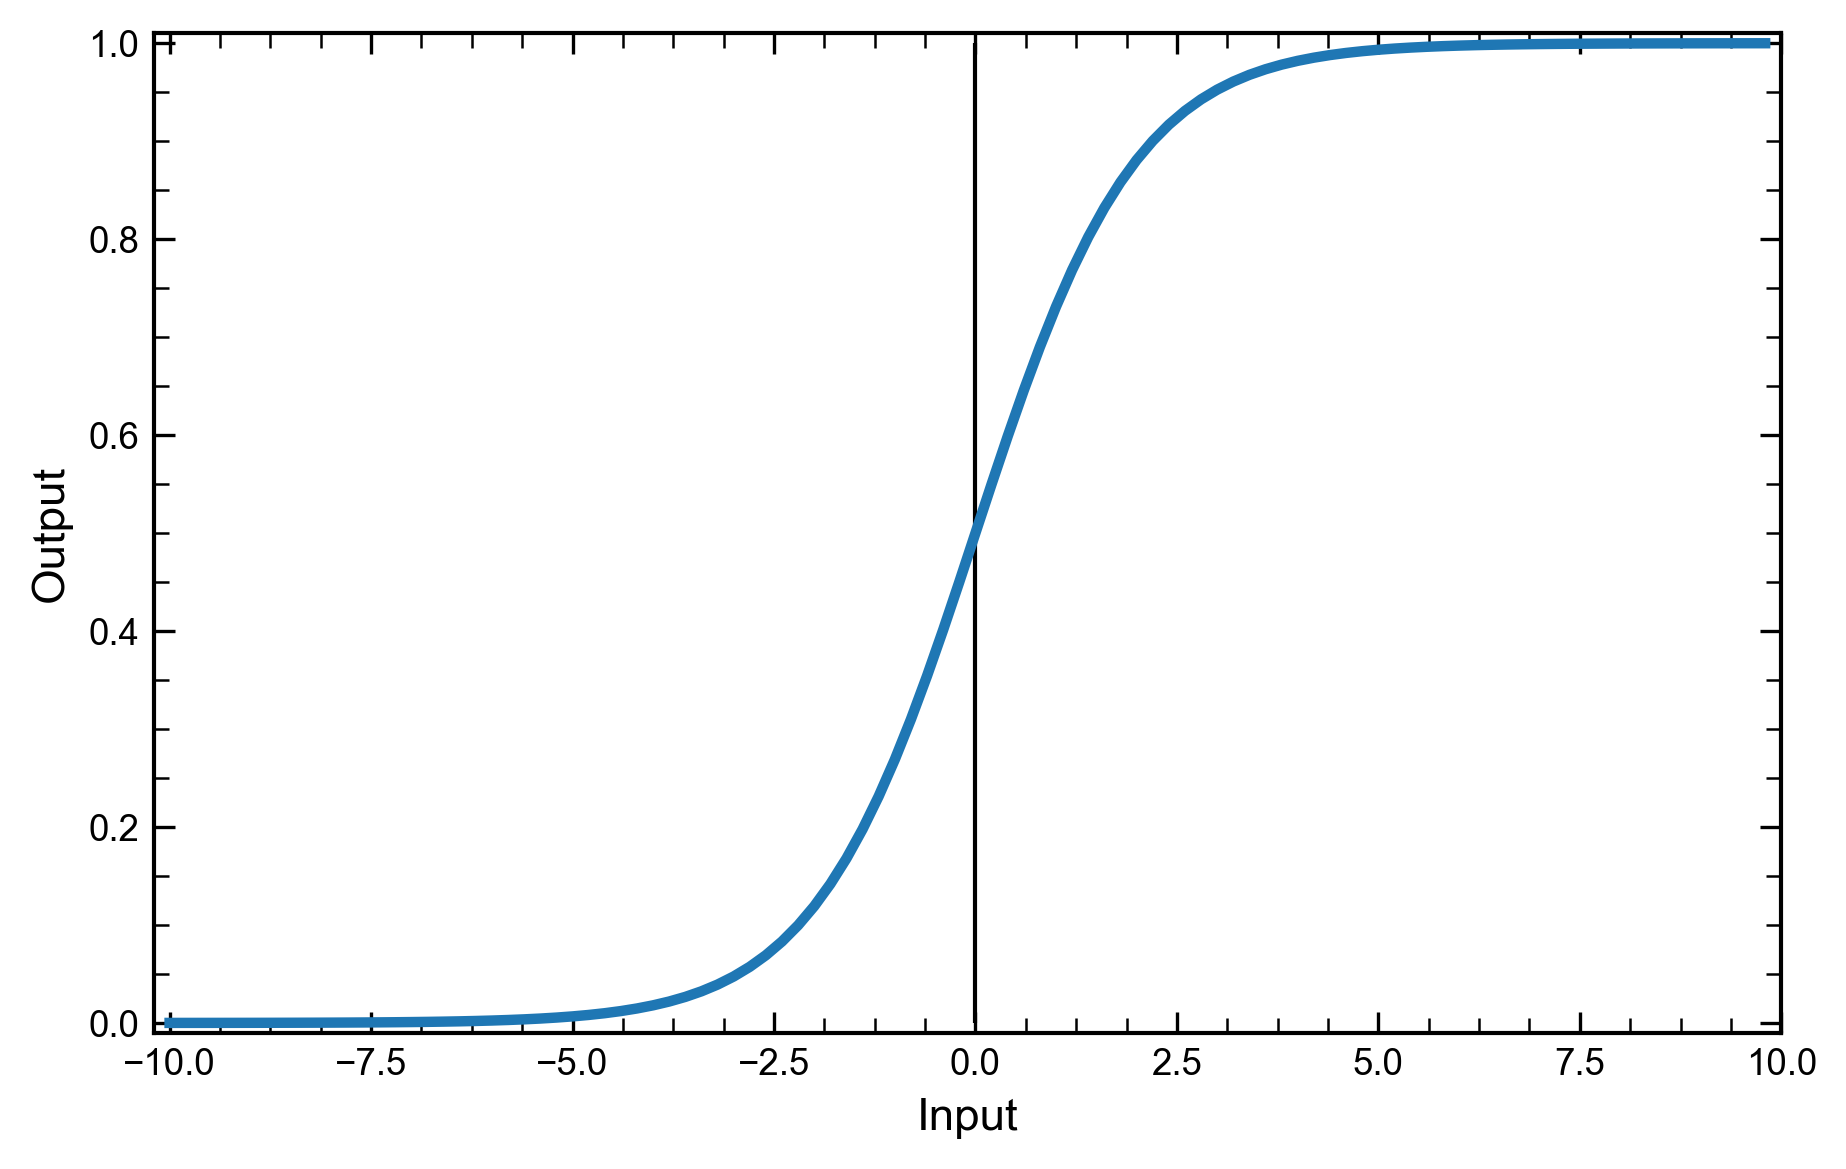
\includegraphics[width=\textwidth]{sigmoid}
        \end{column}
        \begin{column}{0.5\textwidth}
            \begin{itemize}
                \item Bounded, differentiable
                \item Allows for backpropagation
                \item Assigning a single output value $\in (0,1)$
            \end{itemize}
            \begingroup
            \large
            \begin{equation*}
                \frac{1}{1+e^{-s_i}}
            \end{equation*}
            \endgroup
        \end{column}
    \end{columns}
    \begin{itemize}
        \color{red}
        \item Expects only one input value
    \end{itemize}
\end{frame}

\begin{frame}{Categorical final node - Softmax}
    \begin{columns}
        \begin{column}{0.5\textwidth}
            \begingroup
            \huge
            \begin{equation*}
                f(s)=\frac{e^{s_i}}{\sum_j^c e^{s_j}}
            \end{equation*}
            \endgroup
        \end{column}
        \begin{column}{0.5\textwidth}
            \begin{itemize}
                \item Takes an input vector equal to the number of targets
                \vspace{0.1cm}
                \item Sum of vector components is 1
                \vspace{0.1cm}
                \item normalises output to a probability distribution
            \end{itemize}
        \end{column}
    \end{columns}
\end{frame}

\begin{frame}{Loss function - Crossentropy}
    \begin{columns}
        \begin{column}{0.5\textwidth}
            \begin{block}{Binary Crossentropy}
                \begin{equation*}
                    Loss = - \sum_{i=1} y_i \log \hat{y}_i =
                \end{equation*}
                \begin{equation*}
                    -y_1 \log \hat{y_1} - (1-y_1) \log (1-\hat{y}_1)
                \end{equation*}
                \begin{itemize}
                    \item Measures model quality for two classes
                \end{itemize}
            \end{block}
        \end{column}
        \begin{column}{0.5\textwidth}
            \begin{block}{Categorical Crossentropy}
                \begin{equation*}
                    Loss = - \sum_{i=1} y_i \log \hat{y_i}
                \end{equation*}
                \begin{itemize}
                    \item Measures model quality for multiple classes
                \end{itemize}
            \end{block}
        \end{column}
    \end{columns}
\end{frame}
